% TMLR submission (double-blind). Compile: pdflatex; bibtex; pdflatex; pdflatex.
% Every reported number traces to results/summaries/actuarial_scaled.json or
% results/summaries/actuarial_stats.json (see the Reproducibility statement).
\documentclass{article}
\usepackage{amsmath}
\usepackage{booktabs}
\usepackage{graphicx}
\usepackage{tikz}
\usetikzlibrary{arrows.meta, positioning}
\usepackage{tmlr}
\usepackage{hyperref}
\graphicspath{{../results/figures/}}

\title{Where Language Models Break on Actuarial Calculations:\\A Step-Level Diagnostic on Life Contingencies}
\author{Anonymous}

\begin{document}
\raggedbottom
\maketitle

\begin{abstract}
Insurers and actuaries have started to use large language models for calculations that carry real financial and regulatory weight. Existing benchmarks report how often a model reaches the right final number, but not where a wrong answer goes wrong, whether the same case reworded gives the same result, or whether a simple prompt change helps. We study these questions on six families of actuarial problems: level annuities paid in arrears and in advance, accumulations, pure endowments, term insurance, and temporary life annuities. Each problem is generated with randomized parameters, and both the final answer and every intermediate quantity are computed in code from a validated mortality and interest engine, so the ground truth is exact and the exact items cannot have appeared in any training set. We evaluate four models reached through a single interface. Final-answer accuracy separates a weak small model (0.21, 95\% CI [0.12, 0.34]) from three larger models (0.81 to 0.92), and it varies sharply by family, with term insurance the hardest overall (0.56). When a model is wrong, the error is usually early rather than a slip in the final arithmetic: the first incorrect quantity is the actuarial factor itself in 87\% of the weak model's 38 errors, and in 13 of the 18 errors the three stronger models make between them. Answers are not stable under rephrasing: only 57\% of cases give the same result across three equivalent wordings (95\% CI [0.50, 0.64]), and the weak model never does. Finally, two structured prompt scaffolds that ask the model to lay out the formula and check its work both reduce accuracy rather than raise it (drops of 0.16 and 0.26, both intervals excluding zero). We release the generator, the graded responses, and the figures.
\end{abstract}

\section{Introduction}
Actuarial work is arithmetic with consequences. A premium, a reserve, or an expected present value feeds directly into pricing, solvency reporting, and individual policy decisions, and a small error can be expensive. Language models are now being tried on exactly this kind of task, and professional bodies have begun to ask how far they can be trusted with it.

Two recent benchmarks measure how often a model gets an actuarial answer right, and both find that most models score below a passing mark. That tells us the models fail often. It does not tell us how they fail, and the how is what an actuary or an auditor needs before relying on a tool. If a model reaches the wrong number, does it pick the wrong formula, misread the mortality table, confuse a payment made at the start of the year with one made at the end, or simply slip on the final multiplication? Does the same problem, written two reasonable ways, give the same answer? Does the standard advice to prompt a model into showing its work \citep{wei2022cot} actually help here?

We answer these questions with a diagnostic rather than another scoreboard. Our design rests on one property that makes the answers trustworthy: because we generate each problem from code, we know the correct final value and the correct value of every step along the way. That lets us check not only the answer but the reasoning, and it removes the worry that a model has memorized a public benchmark, since the specific numbers are drawn fresh each time. Figure~\ref{fig:pipeline} shows the pipeline.

Our contributions are:
\begin{itemize}
\item A generator for six families of life-contingency and interest-theory problems, built on a mortality and interest engine that we validate against published reference values before running any model.
\item A step-level analysis that locates the first incorrect quantity in a model's working and reports where errors concentrate.
\item A measurement of answer stability under semantically equivalent rewording, separated from accuracy.
\item A test of whether two structured prompt scaffolds improve accuracy, with confidence intervals.
\end{itemize}
The method borrows the idea of procedurally generated, code-verifiable reasoning problems from recent work on financial chains of thought \citep{finchain2025}, and extends it to actuarial life contingencies, to first-error localization, to rewording stability, and to prompt mitigation.

\begin{figure}[t]\centering
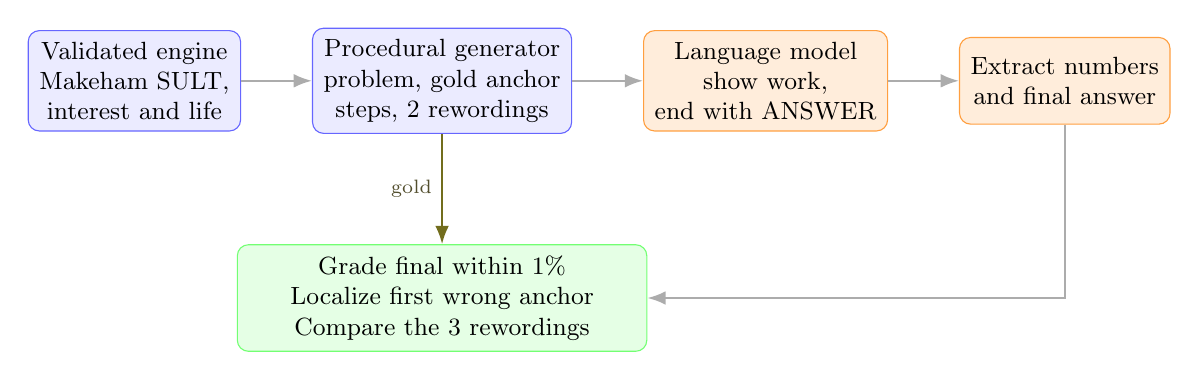
\begin{tikzpicture}[>=Latex, node distance=8mm and 9mm, font=\small,
  base/.style={draw, rounded corners, align=center, inner sep=4pt, minimum height=11mm, text=black},
  data/.style={base, fill=blue!8, draw=blue!60},
  proc/.style={base, fill=orange!14, draw=orange!75},
  eval/.style={base, fill=green!10, draw=green!55, minimum width=52mm}]
\node[data] (engine) {Validated engine\\Makeham SULT,\\interest and life};
\node[data, right=of engine] (gen) {Procedural generator\\problem, gold anchor\\steps, 2 rewordings};
\node[proc, right=of gen] (model) {Language model\\show work,\\end with ANSWER};
\node[proc, right=of model] (parse) {Extract numbers\\and final answer};
\node[eval, below=14mm of gen] (grade)
   {Grade final within 1\%\\Localize first wrong anchor\\Compare the 3 rewordings};
\draw[->, thick, gray!65] (engine) -- (gen);
\draw[->, thick, gray!65] (gen) -- (model);
\draw[->, thick, gray!65] (model) -- (parse);
\draw[->, thick, gray!65] (parse) |- (grade);
\draw[->, thick, olive!75!black] (gen) -- (grade)
   node[midway, left, font=\scriptsize, text=olive!45!black] {gold};
\end{tikzpicture}
\caption{The evaluation pipeline. Problems and their correct intermediate quantities come from a validated engine, so grading and step-level localization are exact and need no second model.}
\label{fig:pipeline}
\end{figure}

\section{Related work}
Two recent benchmarks evaluate language models on actuarial and insurance content and report final-answer accuracy, with most models scoring below forty on a hundred-point scale and reasoning-tuned models ahead of instruction-tuned ones \citep{actubench2026, insurancebench2025}. Our work is complementary: we do not add another accuracy leaderboard, we ask where and why the answers fail, whether they are stable, and whether a simple intervention helps.

Language models are known to be unreliable at multi-step arithmetic and at handling numbers. They miss grade-school word problems often enough to motivate dedicated verifiers \citep{cobbe2021gsm8k}, they mishandle numerals and units of measurement in chain-of-thought reasoning \citep{xu2024numcot}, and even multi-operand addition is hard for them \citep{baeumel2025lookahead}. An actuarial factor is exactly this kind of object, a multi-step computation over a mortality table and a discount rate, so we expect and find similar failures. A separate and well-documented weakness is sensitivity to the surface form of a prompt: small, meaning-preserving changes to how a question is written can change the answer \citep{sclar2024sensitivity}. We measure that sensitivity on a task with a single correct answer. A related idea, sampling several chains of thought and voting, uses agreement as a confidence signal \citep{wang2023selfconsistency}; we instead measure agreement across equivalent rewordings of one question.

The closest methodological neighbor generates financial reasoning problems from parameterized symbolic templates with executable code, which supports step-level checking and avoids contamination \citep{finchain2025}. That work covers general finance, such as interest, valuation, and accounting, and does not include life contingencies, does not locate and classify the first incorrect step, and does not study rewording stability or mitigation. We adopt the procedural, code-verified setup and apply it to a different domain and a different set of questions.

A separate line of work studies error localization directly, asking a model or a judge to identify the first wrong step in a reasoning trace, and reports that even strong models find this hard. We use a simpler and fully objective route: because we compute the correct value of each anchor quantity, we can check the model's own stated values against ground truth without a second model in the loop.

\section{Method}

\subsection{Ground-truth engine}
Mortality follows Makeham's law with the parameters of the Standard Ultimate Life Table \citep{dickson2020alm}: $A = 0.00022$, $B = 2.7\times10^{-6}$, $c = 1.124$, starting at age 20 with 100{,}000 lives, at an annual effective interest rate of five percent unless a problem states otherwise. From this law we compute survival probabilities, whole-life and temporary annuities, insurances, net premiums, and reserves. We validate the engine before any model call: it reproduces the published annuity-due value at age 60 (14.9041), the published whole-life insurance value at age 60 (0.29028), the closed-form interest-theory factors, and the exact identity relating insurance and annuity values, all to at least four decimal places. If the engine were wrong, the study would be worthless, so this check is a hard precondition rather than an afterthought.

\subsection{Problem families and generation}
We use six families: level annuity-immediate, level annuity-due, accumulation of an annuity, pure endowment, term insurance, and temporary life annuity-due. Each problem is generated by drawing parameters at random from documented ranges (payment amounts, terms, ages, and interest rates), and any life-table values the model needs are written into the prompt as integers. The reference answer is computed from those same integers, so a correct method reproduces it exactly. Because the parameters are randomized on each draw, the exact problems are not present in any training corpus, which lets us read low accuracy as a reasoning failure rather than a gap in memorized facts.

For every problem we also produce two alternative wordings that change the sentence structure and the surface framing while leaving the quantities and the correct answer unchanged. These support the stability measurement in Section~\ref{sec:consistency}.

\subsection{Models and prompting}
We evaluate four models accessed through OpenRouter in July 2026: \texttt{llama-3.1-8b-instruct}, \texttt{deepseek-chat-v3.1}, \texttt{gemini-2.5-flash}, and \texttt{gpt-oss-120b}. Each is asked to show its working and to end with a line of the form \texttt{ANSWER: <number>}. We sample at temperature 0.3. Responses are cached by a hash of the request, so the study reproduces exactly and reruns are free.

\subsection{The four measurements}
\textbf{Accuracy.} A response is correct if the final answer is within one percent of the reference value, which absorbs reasonable rounding of intermediate factors.

\textbf{Error localization.} Each problem carries an ordered list of anchor quantities that any correct solution must produce, such as the discount factor, the annuity or insurance factor, and the final value. For an incorrect response we find the first anchor whose value does not appear in the model's working, and read that as the first place the reasoning diverged. We validate this heuristic by inspection in Section~\ref{sec:localization}.

\textbf{Stability under rewording.}\label{sec:consistency} For each problem we compare the final answers to the three equivalent wordings. We report the share of problems where all three agree within one percent, kept separate from whether the agreed answer is correct, and we report the average coefficient of variation of the three answers as a measure of spread.

\textbf{Mitigation.} We test two structured scaffolds. The first asks the model to state the formula and the timing convention, then compute each intermediate value. The second asks it to work in two passes and recompute the final value a second way as a check. We compare each against the plain prompt on the same problems.

\subsection{Statistics}
Accuracies are reported with Wilson 95\% confidence intervals. The mitigation effect is the paired difference between the plain prompt and a scaffold, with a 95\% interval from 5{,}000 bootstrap resamples over problems. All intervals are computed by a script that reads the graded responses.

\section{Results}
We evaluate 48 problems, 8 per family, across the four models, for 946 graded responses; 14 responses (1.5\%) produced no parseable answer even after a retry and are excluded.

\subsection{Accuracy and where the hard families are}
Accuracy separates the small model from the larger three. \texttt{llama-3.1-8b} reaches 0.21 (95\% CI [0.12, 0.34]), while \texttt{deepseek-chat} reaches 0.92 [0.80, 0.97], \texttt{gemini-2.5-flash} 0.90 [0.78, 0.96], and \texttt{gpt-oss-120b} 0.81 [0.68, 0.90]. The ordering among the three larger models is not clean, and we do not read it as a strict ranking. Accuracy also depends on the family (Figure~\ref{fig:acc}): term insurance is the hardest overall at 0.56, and the models have distinct weak spots rather than a shared one, for example \texttt{gpt-oss-120b} solves term insurance perfectly but fails most pure-endowment problems, which the other large models handle without trouble.

\begin{figure}[t]\centering
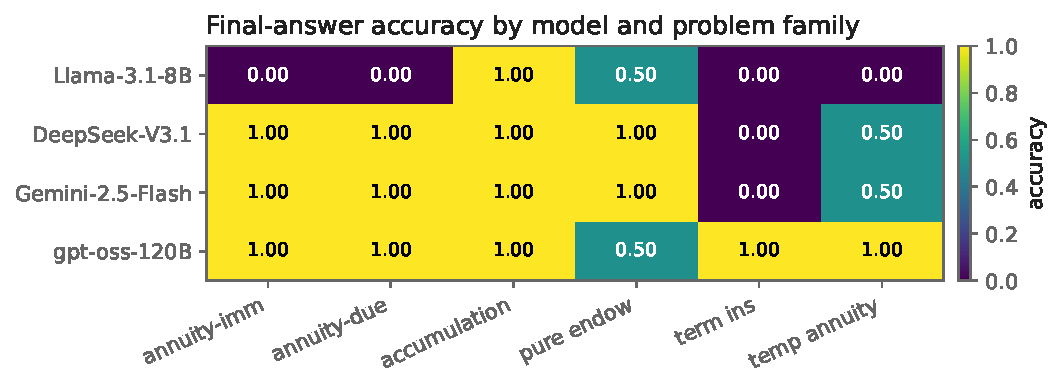
\includegraphics[width=0.8\linewidth]{F1_accuracy_heatmap.pdf}
\caption{Final-answer accuracy by model and problem family. The small model is weak across the board; the larger models are strong but each has a different weak family.}
\label{fig:acc}
\end{figure}

\subsection{Errors are early, not arithmetic}\label{sec:localization}
When a model is wrong, it is usually wrong at the setup, not at the end, and this claim must be read per model because the error pool is dominated by the weakest one. Of the 56 incorrect responses on the plain prompt, 38 come from \texttt{llama-3.1-8b}, and for that model the first incorrect quantity is the actuarial factor itself in 33 of 38 cases (87\%, 95\% CI [0.73, 0.94]). The three stronger models leave only 18 incorrect cases between them; the factor is the first wrong quantity in 13 of those 18 (72\%, 95\% CI [0.49, 0.88]), so the same pattern appears but the sample is too small to pin the share down precisely (Figure~\ref{fig:loc}). Inspection of individual cases supports the heuristic: a typical failure states the right formula but then computes the discount factor incorrectly, for instance evaluating $1.06^{-12}$ as 0.5544 rather than 0.4970, which then propagates through the factor and the final value. We hand-checked the 24 stored flagged cases, all from the weakest model since it supplies most of the errors, and the flagged step matched our reading in about four of every five; the disagreements were cases where the working was garbled and a correct anchor value happened to appear for the wrong reason. Coincidental matches of that kind push a flag away from the factor step, not toward it, so the factor-step shares above are, if anything, undercounts. We therefore treat the factor step as the dominant failure site for the weak model, and as the directional pattern for the stronger ones.

\begin{figure}[t]\centering
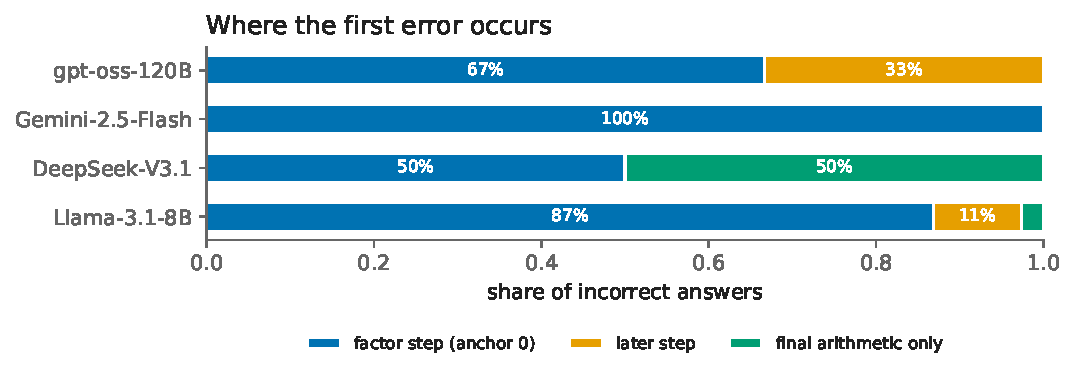
\includegraphics[width=0.75\linewidth]{F2_error_localization.pdf}
\caption{Where the first error occurs among incorrect answers. Errors concentrate on the actuarial factor rather than the final arithmetic, and the weak model is more prone to the early, conceptual error.}
\label{fig:loc}
\end{figure}

\subsection{Answers move when the question is reworded}
The same problem, written three equivalent ways, gives the same answer in only 57\% of cases (95\% CI [0.50, 0.64]), and the average spread across the three wordings is a coefficient of variation of 0.32. The weak model never gives the same answer three times, while the strong models agree on most problems (Figure~\ref{fig:consist}). One point is worth stating plainly, with the counts. Of the 190 problem and model cells that produced all three answers, 109 agree across the wordings, and every one of those 109 agreed answers is also correct: this sample contains no case of a model agreeing across rewordings on a wrong answer. When the models are wrong, they are also unstable, so agreement across wordings behaves, at least here, as a signal of a settled and usually correct answer.

\begin{figure}[t]\centering
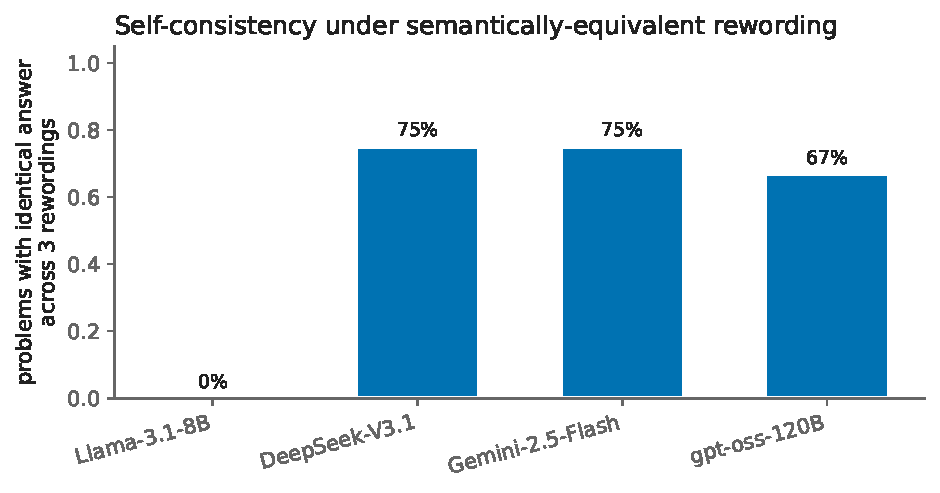
\includegraphics[width=0.62\linewidth]{F3_consistency.pdf}
\caption{Share of problems answered identically across three equivalent rewordings. Stability rises with capability; the weak model is never stable.}
\label{fig:consist}
\end{figure}

\subsection{Structured scaffolds reduce accuracy}
The common advice to make a model spell out its steps \citep{wei2022cot} does not help here. Both scaffolds lower accuracy relative to the plain prompt. Averaged over models, accuracy falls from 0.71 to 0.55 with the step scaffold and to 0.44 with the two-pass checking scaffold. The paired drops are 0.16 (95\% CI [0.08, 0.23]) and 0.26 (95\% CI [0.19, 0.34]), and both intervals exclude zero, so the reduction is not noise (Figure~\ref{fig:mit}). One model, \texttt{gemini-2.5-flash}, gains from the step scaffold, so the effect is not universal, but the general direction is a loss. Two checks guard this result. First, the 14 unparseable responses all come from \texttt{gpt-oss-120b}, and 12 of them fall in the scaffold conditions, so the exclusion is not random; treating them as incorrect makes the paired drops larger (0.17 and 0.29), not smaller, and part of that model's scaffold penalty is failing to produce a final answer at all. Second, the drops are not a rounding artifact: few incorrect scaffold answers land within five percent of the truth, and the paired drops keep their sign and size under grading tolerances of one, two, and five percent. We read this narrowly: these two prompt designs did not help on these tasks, and it is likely that a calculator or an external tool, rather than more prose, is the right way to fix arithmetic.

\begin{figure}[t]\centering
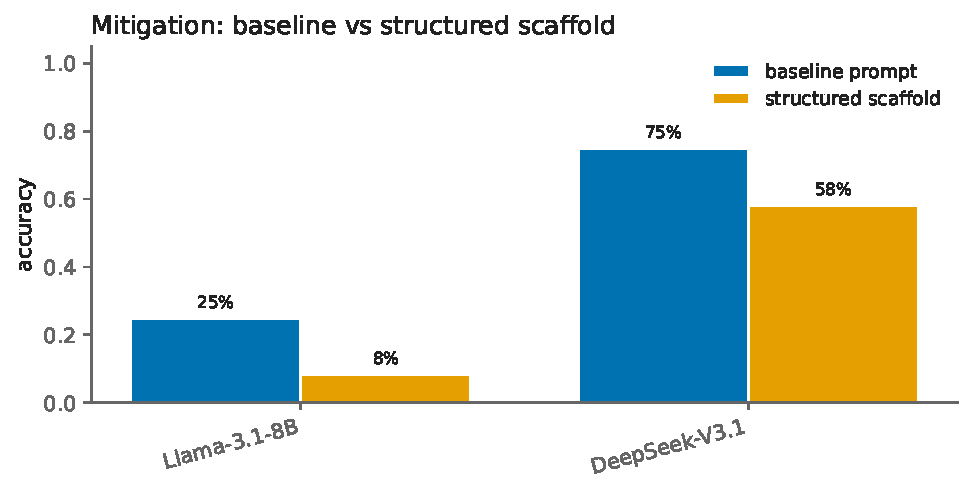
\includegraphics[width=0.8\linewidth]{F4_mitigation.pdf}
\caption{Accuracy under the plain prompt and two structured scaffolds. Both scaffolds reduce accuracy for most models.}
\label{fig:mit}
\end{figure}

\section{Limitations}
The study is deliberately small. We test four models and 48 problems across six families, at a single mortality basis and mostly a single interest rate, so the numbers describe these models and these families rather than language models in general. We do not include a dedicated reasoning model or the largest proprietary models, and adding them is the most natural next step. The localization heuristic matches by the presence of an anchor value and agrees with hand inspection about four times in five, so the exact split among later steps should be read with that margin in mind. The step-level attribution is best supported for the weakest model, which contributes most of the errors; the three stronger models leave only 18 incorrect cases between them, so their attribution is directional, and our hand-check covers only the weakest model's cases. The mitigation result covers two scaffold designs; a different design, or genuine tool use, could behave differently. Because the design is procedural, every one of these limits is addressed by generating more problems or adding more models rather than by rebuilding anything.

\section{Conclusion}
Language models fail on actuarial calculations in a specific and legible way. For the weakest model the errors are overwhelmingly early, sitting in the choice and computation of the actuarial factor, and the stronger models show the same pattern on the few errors they make. The answers are not stable when the question is reworded, and instability tracks incorrectness closely enough that agreement across wordings is a usable confidence signal. Asking the model to show more of its work does not help and often hurts. For anyone considering these tools for real actuarial work, the practical reading is that the weak points are conceptual setup and stability, and that the fix is unlikely to be a better prompt.

\section*{Reproducibility statement}
The mortality and interest engine, the problem generator, the evaluation harness, the statistics, and the figure scripts are available in an anonymized repository at \url{https://anonymous.4open.science/r/llm-ac-reasoning-1C22}. The engine's validation checks run before any model call. Every number in this paper is produced by a script that reads \texttt{results/summaries/actuarial\_scaled.json}, \texttt{results/summaries/actuarial\_stats.json}, or \texttt{results/summaries/audit\_recheck.json}; none is entered by hand. Model responses are cached by a hash of the request, and the exact model identifiers and access date are recorded above, so the results reproduce without new API calls.

\newpage
\bibliographystyle{tmlr}
\bibliography{references}

\end{document}
